\documentclass{standalone}
\usepackage{tikz}
\usetikzlibrary{trees}

\begin{document}

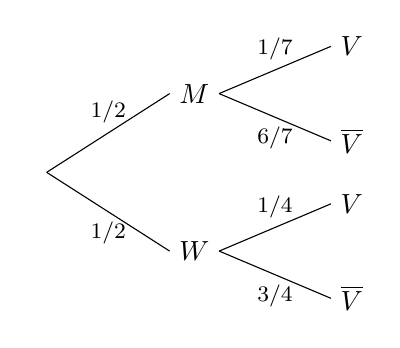
\begin{tikzpicture}[
    grow=right,
    level distance=2.0cm,
    level 1/.style={sibling distance=2.cm},
    level 2/.style={sibling distance=1.2cm},
    edge from parent/.style={draw},
    every node/.style={font=\sffamily},
    edge label/.style={midway, auto, font=\footnotesize},
    parent anchor=east,
    child anchor=west
]
    % Root node
    \node {}
        % Level 1 nodes in reverse order: W, R, B
        child {node {$W$}
            % Children of W in reverse order: R, B
            child {node {$\overline{V}$} edge from parent node[edge label, below] {$3/4$}}
            child {node {$V$} edge from parent node[edge label, above] {$1/4$}}
            edge from parent node[edge label, below] {$1/2$}
        }
        child {node {$M$}
            % Children of B in reverse order: W, R, B
            child {node {$\overline{V}$} edge from parent node[edge label, below] {$6/7$}}
            child {node {$V$} edge from parent node[edge label, above] {$1/7$}}
            edge from parent node[edge label, above] {$1/2$}
        };
\end{tikzpicture}

\end{document}